\section{Minimality e Generation}
Le fasi di \emph{Minimality} e \emph{Generation} sono le ultime due fasi dell'algoritmo. La fase di \emph{Minimality} prendendo come input gli \emph{insiemiC} dalla fase di \emph{Feasibility} genererà sottoinsiemi di pattern minimali. L'output di tale fase sarà input della fase di \emph{Generation} la quale ricaverà, da questi sottoinsiemi, le \textbf{RFD}. La fase di \emph{Generation} non sarà oggetto di studio per questo lavoro di tesi.
\subsection{Nozioni preliminari}
Dalla fase di \emph{Feasibility} si otterranno per ogni RHS un certo numero di insiemi $C_i$ (con $i=1,...,m$) dove ogni $C_i$ sarà composto da un numero di pattern $P_j$ (con $j=1,...,h$) sull'insieme di attributi ($A_1$,...,$A_n$).
\subsection{Minimality}
L'obiettivo della fase di \emph{Minimality} è quello di determinare per ogni insieme $C_i$, generato come output dalla fase di \emph{Feasibility}, quei pattern che siano ammissibili e minimali. Diremo che un sotto-pattern $S_k$, definito come un insieme di attributi per i quali esistono pattern minimali, è ammissibile se quest'ultimo non domina rispetto a tutti gli altri nell'insieme $C_i$. Invece un sotto-pattern $S_k$ è minimale se esiste almeno un sotto-pattern di $S_k$ che non è ammissibile. Inizialmente l'algoritmo per ogni pattern $P_j$ calcola le differenze tra i valori di distanza di $P_j$ e i valori di distanza dei restanti pattern $P_y$ (con $y$ =1, 2, \ldots, h e $y \neq j$).  Ad esempio, considerando il caso in cui il $pattern_j$ sia composto dai valori 6,4,2 rispettivamente per gli attributi A,B,C e $pattern_1 = 3,2,5$ fino ad arrivare a $pattern_h = 1,3,2$, avremo una situazione simile.
\begin{table}[H]
	\centering
	\begin{tabular}{ | l | l | l | l |}
		\hline
		& A & B & C \\
		\hline
		$T_{j1}$ & 3 & 2 & -3\\
		\hline
		. & . & . & .\\ 
		\hline
		. & . & . & . \\  
		\hline 
		$T_{jh}$ & 5 & 1 & -0\\ 
		\hline
	\end{tabular}
 \caption{Esempio di matrice per le distanze tra $P_j$ e $P_y$ in $C_i$}
 \label{tab:table esempio}
\end{table}
Una volta calcolati tali valori e salvati in una matrice $M_{(h,n)}$ l'algoritmo, a partire da quest'ultima, esegue la ricerca dei sotto-pattern minimi seguendo (virtualmente) una struttura denominata \emph{Lattice}. Dato un generico insieme $S$ di $n$ elementi \{A,B,C\}, il \emph{Lattice} è una struttura dati ad albero che ha come radice l'insieme vuoto e come suoi figli i singoli attributi A,B,C. Iterativamente ad ogni livello $i$ dell'albero, si avranno tutte le possibili combinazioni di $n$ elementi di classe $i$.\\
\begin{center}
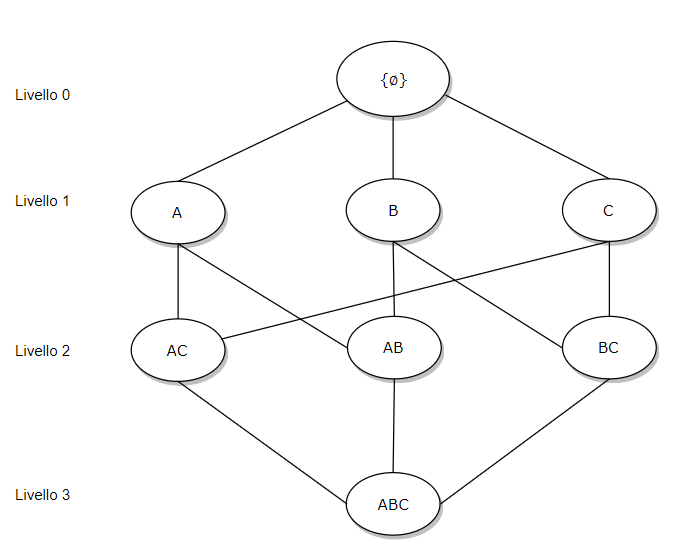
\includegraphics[scale = 0.60]{Immagini/Lattice.png}\\
\end{center}
Per ognuno dei nodi generati l'algoritmo effettua la verifica di minimalità. Definiamo $S_k$ ottimo se valgono le seguenti due proprietà:\\Con $|S_k| = 1$:\\$\bullet$ $\forall$ valore di $t_{jy} \in T_{jy}$ $|$ $t_{jy} \leq 0$.\\Con $|S_k| > 1$:\\ $\bullet$ $\exists$ un valore di $t_{jy} \in T_{jy}$ $|$ $t_{jy} < 0$, oppure $ \forall$  $t_{jy} \in T_{jy}$, $t_{jy}= 0 $.\\ Affinché però si eviti di considerare super-set ammissibili di set minimali oppure, casi in cui nessuna combinazione del sotto-pattern $S_k$ considerato riconduce ad un minimale, applicheremo la tecnica del \emph{Pruning}. Il \emph{Pruning} è una tecnica che riduce le dimensioni degli alberi decisionali rimuovendo sezioni che non riconducono all'ottimo. Definiti tali concetti l'algoritmo, partendo dal livello 1, per ogni nodo dell'albero verifica due condizioni:\\1) Tutti i valori di $S_k$ sono positivi.\\2) Tutti i valori di $S_k$ sono negativi.\\Se si verifica uno solo dei due casi poc'anzi citati l'algoritmo elimina dal \emph{Lattice} tutti gli archi tra il nodo rappresentante $S_k$ e i suoi figli, riducendo così di molto i tempi computazionali. Ritornando all'esempio precedente, con sotto-pattern $S_k = \{A\}$ composto da tutti valori negativi, l'algoritmo elimina gli archi uscenti sui nodi $\{AC\}$, $\{AB\}$, e di conseguenza anche $\{ABC\}$: infine, avendo $S_k$ superato il test di ottimalità, tale sotto-pattern risulta essere minimale.\\
\begin{center}
	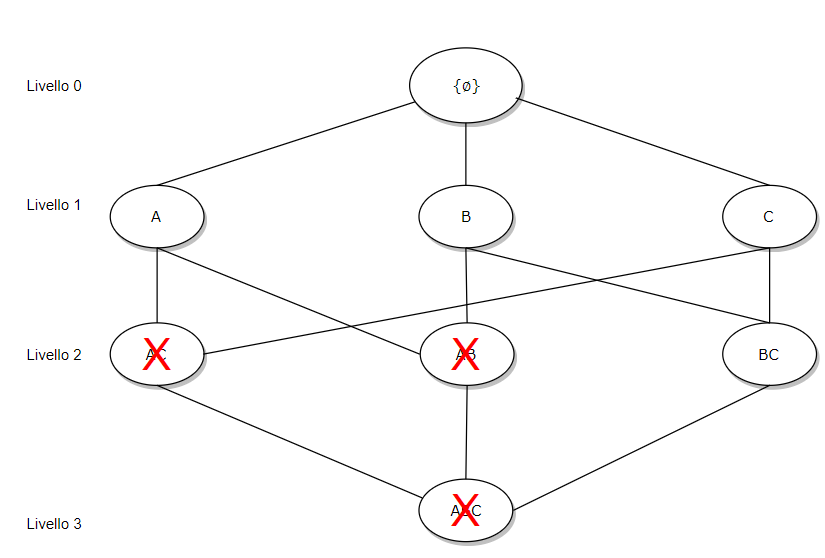
\includegraphics[scale = 0.60]{Immagini/Lattice-taglio.png}\\
\end{center}
L'output del \emph{Minimality} sarà dunque, per ogni pattern $P_j$, i sotto-pattern minimali $S_k$ per quel pattern. Di seguito vengono riportati i pseudocodice dei metodi di MinimalityTest, validate\&PrunePatterns e generateSuperseAttribute.\\
\begin{algorithm}
	\caption{generateSuperSetAttributes(Set \textbf{LevelAttributes}, Set[] \textbf{*columnSet}, Set[] \textbf{*columnEqualSet},)}\label{generatesupersetattributes}
	\begin{algorithmic}[1]	
		
		
		\State Set $\textit{ newLevelAttributes}$
		\State Set[] $\textit{newColumnSet}$
		\State Set[] $\textit{newColumnEqualSet}$
		\State int \textit{codIndex} = 0
		\State column combination \textit{newJ}
		\For{\textbf{each} column combination $j$ in \textit{columnSet/columnEqualSet}}
		\For{\textbf{each} column combination $j'$ in \textit{columnSet/columnEqualSet}
			\State starting from $j+1$}
		\If SAMPREFIX($columnSet[j]$,\textit{columnSet[j']})
		\State \textit{newJ = }GETSUPERSET(\textit{columnSet[j]},\textit{columnSet[j']})
		\State \textit{newLevelAttributes}.ADD($newJ$)
		\State \textit{newColumnSet}[$ccIndex$]=\textit{columnSet[j]}.GETELEMENTS()
		\State U \textit{columnSet[j']}.GETELEMENTS()
		\State \textit{newColumnEqualSet}[$ccIndex$]=\textit{columnEqualSet[j]}.GETELEMENTS()
		\State U \textit{columnEqualSet[j']}.GETELEMENTS()
		\State \textit{ccIndex = ccIndex + 1}	    
		\EndIf
		\EndFor
		\EndFor
		\State \textit{columnSet = newColumnSet}
		\State \textit{columnEqualSet = newColumnEqualSet}\\
		\Return \textit{newLevelAttributes}
	\end{algorithmic}
\end{algorithm}
\begin{algorithm}
	\caption{Validate\&PrunePatterns(Set *\textbf{LevelAttributes}, Set \textbf{*results}, Set[] \textbf{columnSet}, Set[] \textbf{columnEqualSet}, int \textbf{totElements})}\label{validateeprunepattern}
	\begin{algorithmic}[1]	
		
		
		\For{\textbf{each} column combination $j$ in \textit{columnSet/columnEqualSet}}
		\If{\textit{columnSet[j].SIZE() = totElements}}
		\State \textit{results.ADD(columnSet[j])}
		\State \textit{LevelAttributes}.REMOVE(\textit{columnSet[j]})
		\ElsIf{\textit{columnSet[j].}SIZE() + \textit{columnEqualSet[j]}.SIZE() = \textit{totElements}}
		\State \textit{results}.ADD(\textit{columnSet[j]})
		\ElsIf{\textit{columnSet[j].}SIZE() + \textit{columnEqualSet[j]}.SIZE() = \textit{0}}
		\State \textit{results}.REMOVE(\textit{columnSet[j]})
		
		\EndIf
		\EndFor
	\end{algorithmic}
\end{algorithm}
\begin{algorithm}
	\caption{Minimality Test(Set \textbf{C}, int \textbf{numColumn}, int \textbf{numRows})}\label{euclid}
	\begin{algorithmic}[1]	
		\State int[][] $\textit{ diffPatterns} = \text{null }$
		\State int $\textit{ Level} = \text{1 }$
		\State Set $\textit{ LevelAttributes} = \text{}$
        \State Set $\textit{results} = \text{null}$
        \State Set[] $\textit{columnSet} = \text{null}$
        \State Set[] $\textit{columnEqualSet} = \text{null}$

\For{\textbf{each} Set $C_i$ in $C$ in descending order}
\State $\textit{results} = \text{null}$

\For{\textbf{each} pattern tuple $t_p$ in $C_i$}
\State $\textit{diffPatterns} = CREATEDIFFERENCEPATTERNS(t_p)$
\State //fase di inizializzazione

\For{\textbf{each} row tuple $t_j$ in \textit{diffPatterns}}
\For{\textbf{each} column $j$ of $t_j$}
\State \textit{levelAttributes}.ADD($j$)
\EndFor
\For{\textbf{each} value $e$ in column of $t_j$}
\State \textit{e} = \textit{diffPatterns.GETELEMENT($j$)}
\If \textit{e} = 0
\State \textit{columnEqualSet[$j$].ADD($e$)}
\Else{\textbf{ if }$e < 0$}
\State \textit{columnSet[$j$].ADD($e$)}
\EndIf
\EndFor
\EndFor
\State //fine inizializzazione
\State //fase di ricerca via lattice
\While{\textit{level}$<=$\textit{ numColumn}}
\State VALIDATE\&PRUNEPATTERNS(\textit{*LevelAttributes,*results,
\State columnSet,columnEqualSet,numRows})
\State \textit{Level = Level + 1}
\State \textit{LevelAttributes = }
\If{\textit{LevelAttributes}.SIZE() = 0}
\State \textbf{break}
\EndIf
\EndWhile
\State //fase di ricerca via lattice
\EndFor
\State GENERATED(\textit{results}) //fase descritta nella tesi Leo
\EndFor
	\end{algorithmic}
\end{algorithm}